\chapter{Pin Control Defense}
\label{chap:defense}

This chapter proposes a possible countermeasure to Pin Control Attack.
First, it describes the overall design of Pin Control Defense, showing different approaches to tackle the attack at different levels
and explaining our design choices. Second, it contains a detailed report of the defense implementation.


\section{Design}
We report the design phase below, starting from a preliminary analysis of the problem to a discussion of different possible solutions.
Then, a detailed description of the defense architecture concludes the section.


\subsection{Preliminary analysis}
\label{sec:pre_analysis}

The main goal of our defense is to detect Pin Control Attack while being able to not consume the limited resources inside the target system,
and to not affect real-time operations. The timing of the operations is fundamental in systems like PLCs, on which the minimum delay may alter the physical process.

We make the same assumptions contained in the threat model of \mysec{sec:threat_model}.
Therefore, we assume that the system, and our defense as well, is protected by the previously discussed HIDSs.
Starting from the analysis reported in \mychap{chap:attack}, we identify the I/O configuration as the main resource we aim to protect from Pin Control Attack.
To target I/O configuration, the attacker may use other system capabilities, such as virtual address mapping and debug registers.
Before describing our defense approach, we define the following components of a SoC:
\begin{itemize}
	\item \itemname{I/O subsystem}: the set of all the control registers actively used by the SoC, whose unathorized modification may have direct or indirect
		effects on the controlled process. The values contained inside these registers represent the I/O configuration.
		In particular, we are interested into pin control registers, which directly determine the behaviour of the SoC I/O pins.
		However, a SoC typically contains many devices and controllers which may be in charge of a subset of I/O pins. In other words, some pins
		can be multiplexed to specifical devices inside the SoC. Since these devices are programmed through their own control registers,
		altering these registers may indirectly affect I/O pins as well. Thus, both pin control registers and device control registers
		are considered as part of the I/O configuration. The attacker who has knowledge of the system and its I/O peripherals may access
		all these registers to alter the physical process.
	\item \itemname{Debug subsystem}: the SoC subsystem that enables debug capabilities for the operating system and its processes.
		Typically, it consists of a set of registers, called \emph{debug registers}, inside the processor of the SoC.
		The operating system may provide an interface to access them, both for kernel side and user side.
		The attacker may leverage the debug subsystem to obtain accurate timing information and conduct more sophisticated attacks,
		either using the interface provided by the operating system or the low-level processor instructions directly (depending on its privilege level).
	\item \itemname{Mapping subsystem}: the system that manages mappings between physical and virtual addresses, both for kernel and user space.
		It is typically supported by the Memory Management Unit (MMU) in hardware, and by the operating system in software. Within the context of a PLC,
		the runtime may use this subsystem to configure the I/O and to perform read/write operations. An attacker can access physical I/O addresses
		(thus, I/O configuration) either by requesting a new mapping to the system or by using an already existing mapping.
\end{itemize}

In order to choose the strategy to detect Pin Control Attack, we compared different approaches, as proposed in \cite{ghostplc}:
\begin{enumerate}
	\item monitoring I/O configuration to detect changes;
	\item monitoring the use of debug registers;
	\item monitoring the mapping requests targeting I/O configuration;
	\item monitoring performance overhead;
	\item using a trusted execution environment.
\end{enumerate}
These approaches are not mutually exclusive, and may be used simultaneously to get a higher protection level.
In this work, we designed and implemented the first three approaches in combination. A discussion about this design choice is reported in \mysec{sec:def_arch}.
Our solution, however, may be extended to include the last two approaches as well, which we briefly discuss in the following sections.


\subsubsection{Monitoring performance overhead}

A detection system based on performance monitoring may be useful to add a further protection, especially against the attack variant
which uses debug registers. In general, such a monitor would be also useful for other kind of attacks targeting PLCs, because these systems cyclically performs
a limited amount of well-known operations. This simplifies the detection of any deviation from the standard behaviour.
In our case, a performance monitor would be helpful to cover those attacks that the first three strategies are not able to detect,
although, as discussed in the following sections, those are very limited cases.
Deploying a performance monitoring system, anyway, does not require very high effort because it can leverage \emph{Hardware Performance Counters} (HPC),
nowadays available in almost all the SoC processors. The most challenging part would be, of course, integrating the monitor with the PLC runtime.
When a new logic is uploaded, a burst of operations are executed, and they must be excluded from the detection. Furthermore, a new logic may perform different operations
with respect to the previous one; therefore, the monitor should be able to recognise the event and update its statistics as well.


\subsubsection{Trusted execution environment}

A Trusted Execution Environment (TEE) is a particular set of hardware and software components providing security features,
such as isolated execution, integrity of Trusted Applications (TAs), and integrity and confidentiality of TAs assets \cite{tee}.
The TEE technology is based on the concept of partitioning a computing system into Secure and non-Secure world, where
the code running into non-Secure world cannot access the Secure partition.
A lot of effort has been put into the standardisation of the TEE, and some commercial solutions already exist,
such as Intel Trusted Execution Technology (TXT) \cite{intel_txt} and ARM TrustZone \cite{trustzone}.
Since embedded systems are our main target, we provide a brief description focused on the ARM TrustZone implementation.
In this technology, the physical memory is partitioned into Secure and non-Secure regions, and the processor core is divided into Secure and Non-secure virtual cores.
The virtual core is distinguished by the NSTID (Non-Secure Table IDentifier) bit associated with the current instruction,
while each instruction or data address (\ie each bus transaction) is marked with an NS bit.
The protection of the Secure world is guaranteed by checking all the accesses to memory or peripherals.
The Non-secure core can only access Non-secure memory regions, while the Secure world can use both Secure and Non-secure addresses.
This partitioning is parallel and independent from Supervisor/User modes available on the CPU. Therefore, each world has its own supervisor and user mode as well.
To improve the performance of this architecture, TLBs and caches may support the NS attribute for each entry as well.
This enables Secure and Non-secure entries to co-exist avoiding TLB and cache flushes on every switch between the two worlds.
The switching between Secure and Non-secure world is managed through a specific Secure Monitor Call (SMC) instruction,
which changes the core mode into Monitor Mode. The code executed into monitor mode is always Secure, and it basically performs the context switch
between the two virtual cores. If a Secure process is loaded, the core NS-bit is set accordingly.
Since the Secure world may contain a whole parallel micro-kernel with trusted user applications, it may be possible
to deploy Pin Control Defense inside the trusted domain, protecting the defense itself from defense-aware attackers.
However, the overhead imposed by a trusted execution environment may be unacceptable for embedded systems with real-time constraints like PLCs.


\subsection{Defense Architecture}
\label{sec:def_arch}

Based on the previous considerations, we designed a defense which is able to detect Pin Control Attack at three different levels.
Its overall architecture is shown in \myfig{fig:defense}.
\begin{figure}[h]
\centerline{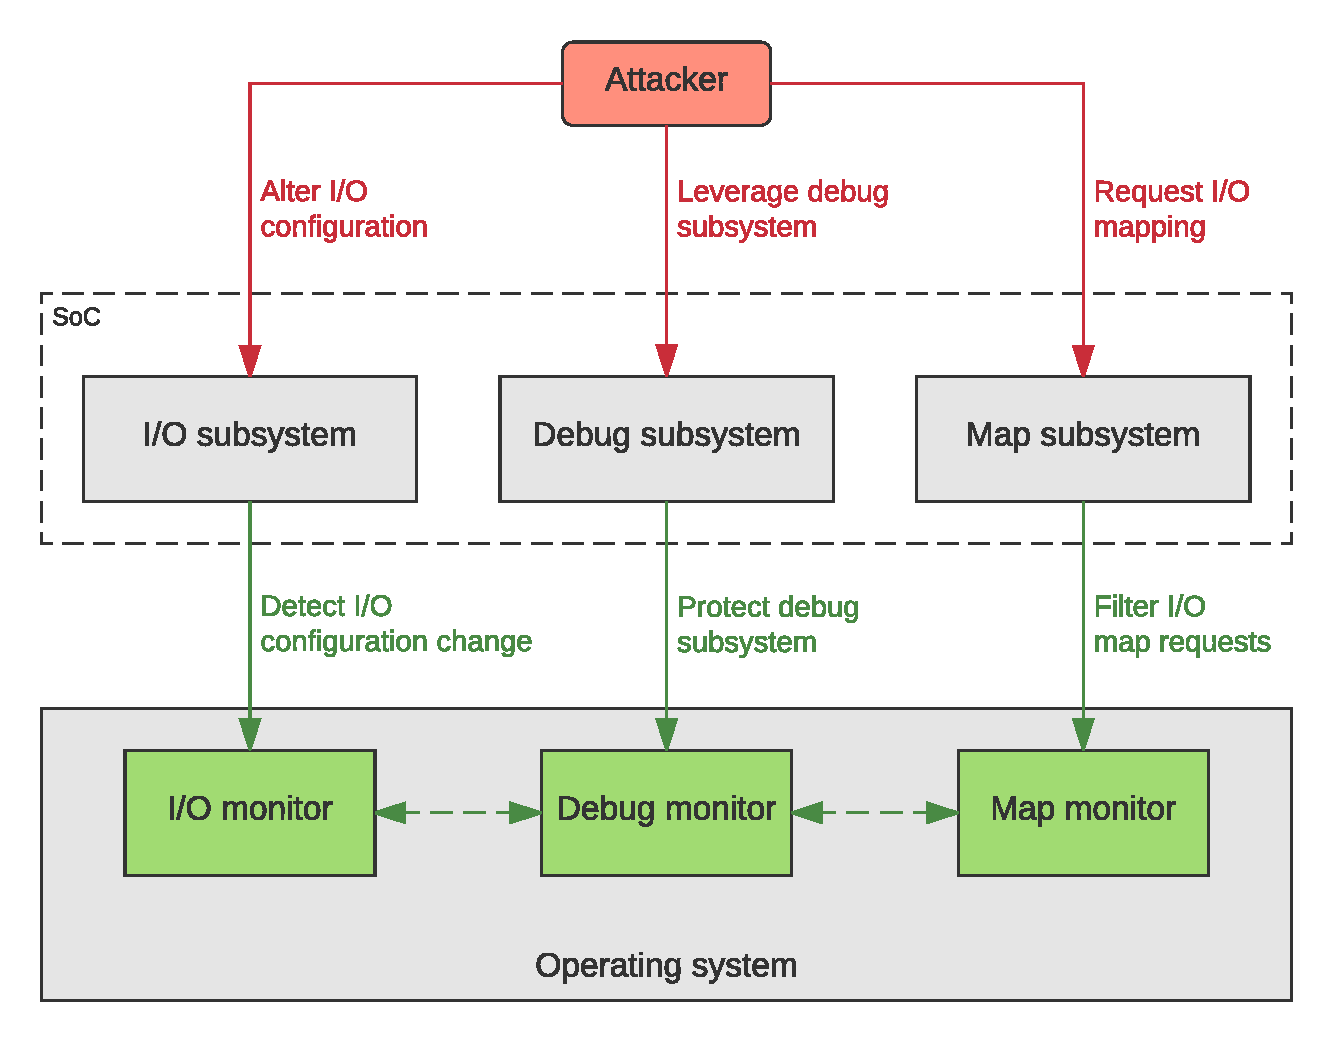
\includegraphics[width=0.8\textwidth]{res/defense}}
\caption{ \label{fig:defense}}
\end{figure}
Considering that the attacker can possibly follow any of the paths highlighted in red in \myfig{fig:defense},
our monitoring system has been divided into three main components deployed alongside the operating system:
\begin{itemize}
	\item \itemname{I/O monitor}: its purpose is to watch the I/O configuration and detect any malicious change.
	\item \itemname{Debug monitor}: it aims to protect the debug subsystem from malicious usage.
	\item \itemname{Map monitor}: it acts as a filter for mapping requests targeting I/O memory.
\end{itemize}

These monitors are responsible for reporting detection information related to interesting events of the respective subsystems.
The reported events are not necessarily due to Pin Control Attack. In particular, the I/O monitor should decide whether a particular I/O modification
can be considered legitimate or not. Debug and map monitors, instead, serve at least the following purposes:
\begin{itemize}
	\item \itemname{early detection}: the attack can be detected before it modifies the I/O configuration;
	\item \itemname{raising the bar}: they limit the attacker possibilities, by restricting the access to the corresponding subsystem;
	\item \itemname{logging}: they provide additional information, useful to figure out how an eventual attack has been conducted.
\end{itemize}
Since these modules are designed to be customizable, the effects depends on their actual configuration.
The following sections describe in more detail the design and the role of each module.


\subsubsection{I/O monitor}

The I/O monitor plays the most critical role into our detection system.
Its main task is to cyclically check the values contained into I/O configuration registers, to verify that they are conforming with the logic currently loaded into the PLC.
If a change into a target register has been detected, it determines whether this modification is legal or not, according to a given trusted behaviour.
As discussed in \mysec{sec:plc_arch}, a new I/O configuration may come with a new PLC logic, and the PLC runtime must be able to apply the change without
having our defense to interfere.
Therefore, an automated mechanism able to distinguish between trusted and malicious configurations is needed.
This is not an easy problem, because an optimal solution would require an authentication between PLC runtime and I/O subsystem,
and this is not reasonable in our highly constrained system.

To tackle this problem, we designed the following strategy, which we used to implement the I/O monitor:
\begin{enumerate}
	\item define a trusted behavioural model of the I/O configuration;
	\item \label{enum:io_monitor} constantly monitor the I/O configuration to detect possible modifications;
	\item if a change is detected, verify whether it is conforming to the defined behaviour or not;
	\item if it is, accept the new configuration and go back to \ref{enum:io_monitor};
	\item otherwise, it is probably Pin Control Attack: react according to the configured monitor action and go back to \ref{enum:io_monitor}.
\end{enumerate}
To define the behavioural model, it is required to determine the set of configuration registers actively used into the target system,
\ie the set of registers that may affect the physical process. Then, for each register (or for each bit of each register if necessary),
the model should define under which conditions the corresponding value may change. These conditions are highly dependent on the target implementation.
Generally speaking, they can be represented by simple time constraints (\eg the value cannot change twice within $\SI{20}{ms}$),
logical conditions (\eg the value must be conforming to the running PLC logic), a statistical model, or a combination of these.
Each condition can either provide an exact distinction between a trustworthy and a malicious modification (typically logical conditions),
or a heuristic only.

An important parameter to discuss is the time interval of the main monitor loop. Since no other mechanisms are provided by the hardware,
such as interrupts, we can only detect I/O configuration changes by cyclically checking its current values. Greater scanning intervals may give the attacker
enough time-window to reach its purpose. For instance, given a PLC scan cycle of $\SI{10}{ms}$ and a monitor interval of $\SI{50}{ms}$,
if the attack is able to synchronise itself with the monitor loop, it has enough time to alter $\left \lfloor{\frac{\SI{50}{ms}}{\SI{10}{ms}}}\right \rfloor = 5$ consecutive I/O operations
and then restore the configuration back before getting noticed. Smaller intervals, instead, may cause too much performance overhead.
We provide our experimental results in \mychap{chap:results}.

Another challenging aspect of this approach is to decide which action the monitor should follow if an attack has been detected.
We distinguished at least three main reactions for I/O monitor:
\begin{itemize}
	\item report the event to the system;
	\item revert the configuration back to the last known before the attack;
	\item stop the control process.
\end{itemize}
The choice among these actions (or a combination of them) again depends on the target implementation.
Typically, reporting the event is the minimum that the monitor can do, while other reactions should be decided according to risk associated with the physical process
and to the monitor reliability. If a detection is proven to be correct, due to an exact condition,
then reverting the configuration back could be the best choice. Otherwise, if the detection condition is a heuristic and the risk is critical,
stopping the control process may be considered as a more cautious alternative.
In general, if a monitor only reports about events we call it \emph{passive}, otherwise it is an \emph{active} monitor.


\subsubsection{Debug monitor}

This monitor is responsible for protecting the debug subsystem from malicious usage. Debug registers may be used by the attacker to gain accurate timing
information about the PLC logic I/O operations.
Similarly to what the I/O monitor does, the debug monitor continuously watches the values contained into debug registers to detect malicious modifications.
In our design, we assumed that there is no need to use debug registers into the target PLC if it is already deployed into a real control system.
As confirmed by our experiments, they are actually never used.
Typically, the SoC debug subsystem may only be needed by PLC vendors during design and implementation of their own product.
Since the operating system may provide user level access to debug registers (\eg \verb|ptrace| API on Linux), we can simply disable this user interface.
However, there is no mechanism to permanently disable debug registers also at kernel-wide level.
To understand this problem, we need to distinguish the following two cases: the debug support can be either enabled or disabled into the kernel itself.
If it is enabled, the attacker may simply leverage the system interface to use debug registers from kernel space.
If debug support is disabled, an attacker who gains kernel level access (as in kernel module version of Pin Control Attack) can always re-enable them at run-time
by inserting its own debug exception handler into the OS interrupt vector table (see \cite{arm-evt,x86-idt}).
However, this kind of attack is already covered by the defenses assumed in our threat model, because it is a data hooking technique.
Thus, we designed the following monitor strategy, that is required only if debug support is enabled into the operating system:
\begin{enumerate}
	\item disable debug registers user space interface;
	\item \label{enum:debug_monitor} constantly monitor debug registers to detect possible modifications (from kernel space);
	\item if a change is detected, it is Pin Control Attack: react according to the configured monitor action and go back to \ref{enum:debug_monitor}.
\end{enumerate}
The strategy is (in part) a simplification of the I/O monitor approach, on which the trusted behavioural model assumes that debug registers never change in a production system.
Based on this assumption, the debug module allows our defense to provide an early detection of the attack, before I/O configuration is actually altered.
The discussion about the monitor time interval is the same as for the previous I/O monitor: a trade-off between attacker time-window and monitor overhead.

When an attack has been detected, restoring the previous values of debug registers is surely the best action to take,
because the assumption ensures that only malicious changes may occur.
Halting the PLC process, instead, is certainly not needed because the control process is not directly affected by a modification of the debug subsystem.
In any case, the event is reported to the system. To uniform the design, the debug monitor can be configured either as passive or active,
although the passive mode is strongly discouraged for the above reasons. If the monitor is active, it actually raises the bar for the attacker,
who cannot leverage debug registers anymore.


\subsubsection{Mapping monitor}

As discussed in \mysec{sec:pre_analysis}, the attacker may either request a new mapping between physical and virtual memory, or re-use an existing one before
modifying I/O configuration. The map monitor leverages this fact, providing a further detection mechanism usable in combination with the previous two.
Typically, the operating system provides an interface, for user space, through which each process can map a physical address region to a corresponding virtual region.
In the following part of this document we refer to it as ``mapping interface''.
The actual mapping is performed inside the kernel, and the process receives a valid virtual address as result.
The attacker can leverage this mechanism to gain access to the I/O configuration registers from user space.
According to the implementation, the PLC runtime may use this mechanism as well, and if it does, the attacker may try to re-use the PLC runtime virtual address.
We distinguish at least two techniques to re-use existing virtual addresses:
\begin{itemize}
	\item exploit a remote code execution vulnerability on the PLC runtime owning the addresses;
	\item set debug register on PLC runtime virtual address (the debug handler will have access to the process virtual addresses).
\end{itemize}
We exclude the second technique, because it is already detectable by the debug monitor. The first one, instead, can only be counteracted by detecting the control flow attack itself.
Thus, the aim of this monitor is not to detect addresses re-using, which is out of our scope, but to monitor \emph{new} mapping requests.
To achieve the goal, we dynamically replace the functions belonging to the mapping interface with our own versions (hook).
We can summarise the strategy of the map monitor as follows:
\begin{enumerate}
	\item \label{enum:map_model} define a trusted behavioural model for I/O mapping requests of the PLC runtime;
	\item hook all the functions belonging to the mapping interface;
	\item at each new mapping request, verify whether the requested physical address range overlaps the I/O configuration region or not;
	\item if there is no overlap, forward the request to the original system function;
	\item if an overlapping region is detected, verify whether the request is conforming to the trusted behaviour or not;
	\item if it is, forward the request to the original system function;
	\item if it is not, it is probably Pin Control Attack: react according to the configured monitor action.
\end{enumerate}
The behavioural model of step \ref{enum:map_model} should describe if and how the mapping interface is used by the PLC runtime.
We analysed the behaviour of our target systems, with the following results:
\begin{itemize}
	\item Raspberry Pi: the CODESYS runtime un-maps and re-maps the I/O every time a new PLC logic is uploaded;
	\item Wago PLC: e!RUNTIME never maps physical I/O from user space, because it is managed by the system driver.
\end{itemize}
The next step of the strategy, function hooking, must satisfy at least the following requirements (see implementation in \mysec{sec:def_impl} for more details):
\begin{itemize}
	\item it must be efficient: mapping functions may be called many times by processes (\eg in Linux, they are used not only to map physical memory,
		but any file, device, etc.);
	\item considering the threat model discussed in \mysec{sec:threat_model}, it must be applied before the Autoscopy Jr. detection system is deployed;
		otherwise, our modification will be considered as malicious.
\end{itemize}

Finally, the reaction of the map monitor to an eventual detection depends on the PLC runtime behaviour. If the PLC runtime maps the I/O (as in Raspberry Pi),
then a mechanism to distinguish between good and malicious requests is needed. To accomplish this, we may list the following alternatives:
\begin{itemize}
	\item heuristic approach based on statistical data;
	\item integration of the defense with the PLC runtime.
\end{itemize}
Since the first approach cannot give an exact detection, the monitor may simply report the detection to the system.
The second approach, instead, may be implemented in different ways. For instance, the map monitor could provide a separate mapping interface
reserved only for the PLC runtime process.
In any case, if the system allows to have an exact detection mechanism, the monitor may directly deny the malicious request, factually raising the bar for the attacker.


\section{Implementation}
\label{sec:def_impl}

TODO Pin Control Defense implementation.
